\chapter{System Architecture}
\section[Introduction]{Introduction}

The main challenge for the development of CubeSats is to fit all the necessary equipment within the standard frame size while meeting the weight constraints. The EPS design is crucial for the successful CubeSats mission, which needs to consider several factors such as mission duration, orbit altitude, inclination angle, size of PV panels and its arrangement, load profile, volume and weight limits, radiation effects, overall efficiency, simplicity of control, component count, flexibility in battery configuration, reliability, and fault-tolerant capability. 
\\ 
One of the important steps in EPS design is the selection of most suitable EPS architecture. The different types of CubeSat EPS architectures are shown below.
\\ 
\begin{figure}[H]
	\centering
	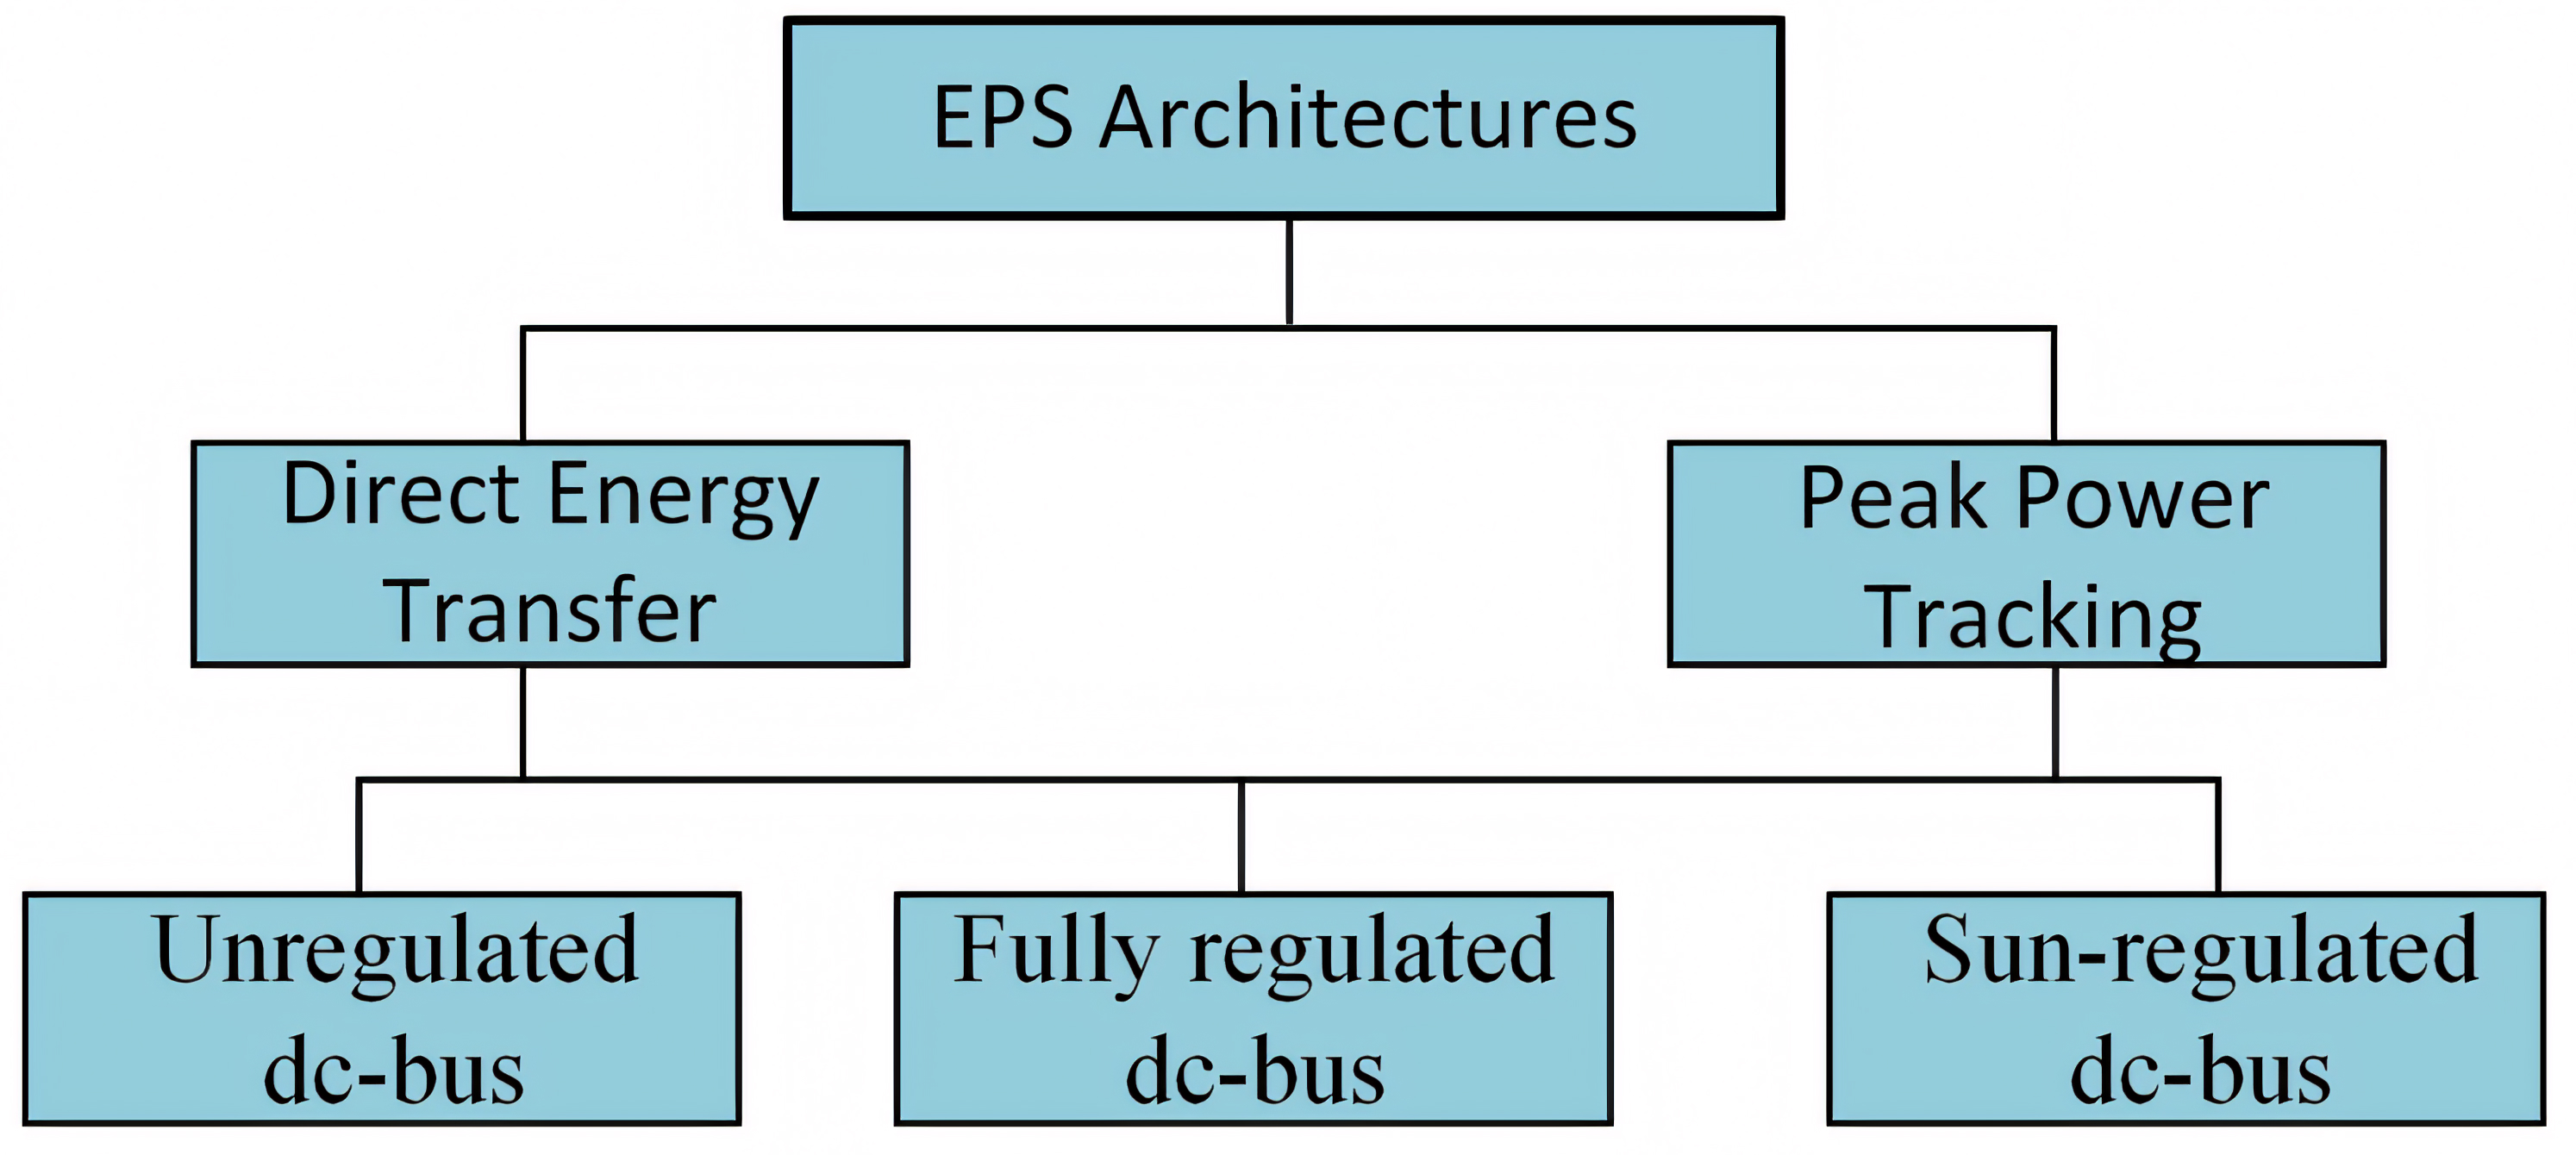
\includegraphics[width=0.7\columnwidth]{IMGS/EPSarchitectures.jpg}
	\caption{CubeSat EPS architectures}
	\label{fig:arch}
\end{figure} 
\\ 
Based on the interfacing of PV panels, the EPS architectures are classified as direct energy transfer (DET) and peak power tracking (PPT) architectures. 
\\ 
In the DET architecture, the PV panels are directly connected to the battery and/or load equipment via diodes. It also uses a shunt regulator in parallel with the PV panels to absorb excess power when the battery reaches full-charge condition.
\\ \\
 In the PPT architecture, the PV panels are interfaced with a power electronic converter to extract the maximum power from the panels under widely varying operating conditions such as solar irradiation, PV panel temperature, and inclination angle. 
 \\ 
The DET architecture requires matching of PV panel characteristics and the dc-bus voltage to generate maximum possible power which is not straightforward in the space missions. Therefore, the majority of CubeSats utilize the PPT architecture to maximize the solar energy harvest, which has limited PV panel capacity and storage capacity due to strict volume and weight constraints. 
\\ \\
The PPT architectures are further classified based on dc-bus voltage regulation: unregulated dc-bus, regulated dc-bus; and sun-regulated dc-bus. 
\\
The unregulated dc-bus EPS architecture has the battery terminals directly connected to dc-bus. When the battery voltage reaches its upper limit, the MPPT converter is operated in voltage regulation mode to avoid further charging of the battery. 
\\ 
The regulated dc-bus EPS architecture interfaces the battery with a dc–dc converter to maintain the dc-bus voltage at the predefined value. This architecture enables the operation of CubeSat at higher dc-bus voltage so that conduction and ohmic losses are reduced. 
\\
In the sun regulated dc-bus EPS architecture, the dc-bus voltage is maintained at reference value only during the sunlit period. During the eclipse period, the battery gets connected to the dc-bus via a diode to supply the loads.

\section[Selected Architecture]{Selected Architecture}



The electrical power system (EPS) is a critical component of CubeSat architecture, as it provides power to all the satellite's systems and payloads. EPS architecture of a CubeSat is designed to be highly efficient and reliable, while minimizing the mass and power consumption of the components. The EPS must be carefully designed and tested to ensure that it can withstand the harsh space environment and meet the mission requirements.\\

The CubeSat is equipped with six solar panels on each side. To ensure that the solar panels operate at their most efficient points, the solar panels are connected to MPPT ICs such that the solar panels on the opposite sides are connected to single MPPT IC. Since only one of the opposite sides of the cube is irradiated at any time, the MPPT of two solar panels can be achieved using a single IC. This arrangement reduces the number of MPPT ICs required by the system. The MPPT runs a constant voltage algorithm and delivers 5 V at the bus. 
\\

When the CubeSat is capable of generating enough power through the solar panels, the components are directly powered by the panels through the bus. At the same time, a battery charging IC uses some of the energy to recharge the Li-ion cell. The battery charger takes the 5V from the bus and converts it to the voltage and current optimal for battery charging depending on the state of charge, temperature of the cell etc.During eclipse the battery power the energy from the panels is absent and the battery powers the CubeSat components. The voltage of the battery varies from 3.7 V to 4.2 V.
\\

The buck and boost converters provide power to the 3.3 V and 5 V rails respectively. Their input voltage varies from 3.6 V to 5 V to account for direct power from the panels when sunlight is available and for battery power during eclipse.
\\

To ensure proper functioning and to identify any faults in the system, there are various voltage and current measurement units placed at various points in the circuit. They measure the current and voltage at each point and the data is fed to a micro-controller, which is programmed to open the switches at the rails in case of any faults. The system architecture is shown in figure \ref{fig:mainarch}.

\begin{landscape}
	\begin{figure}[h]
		\centering
		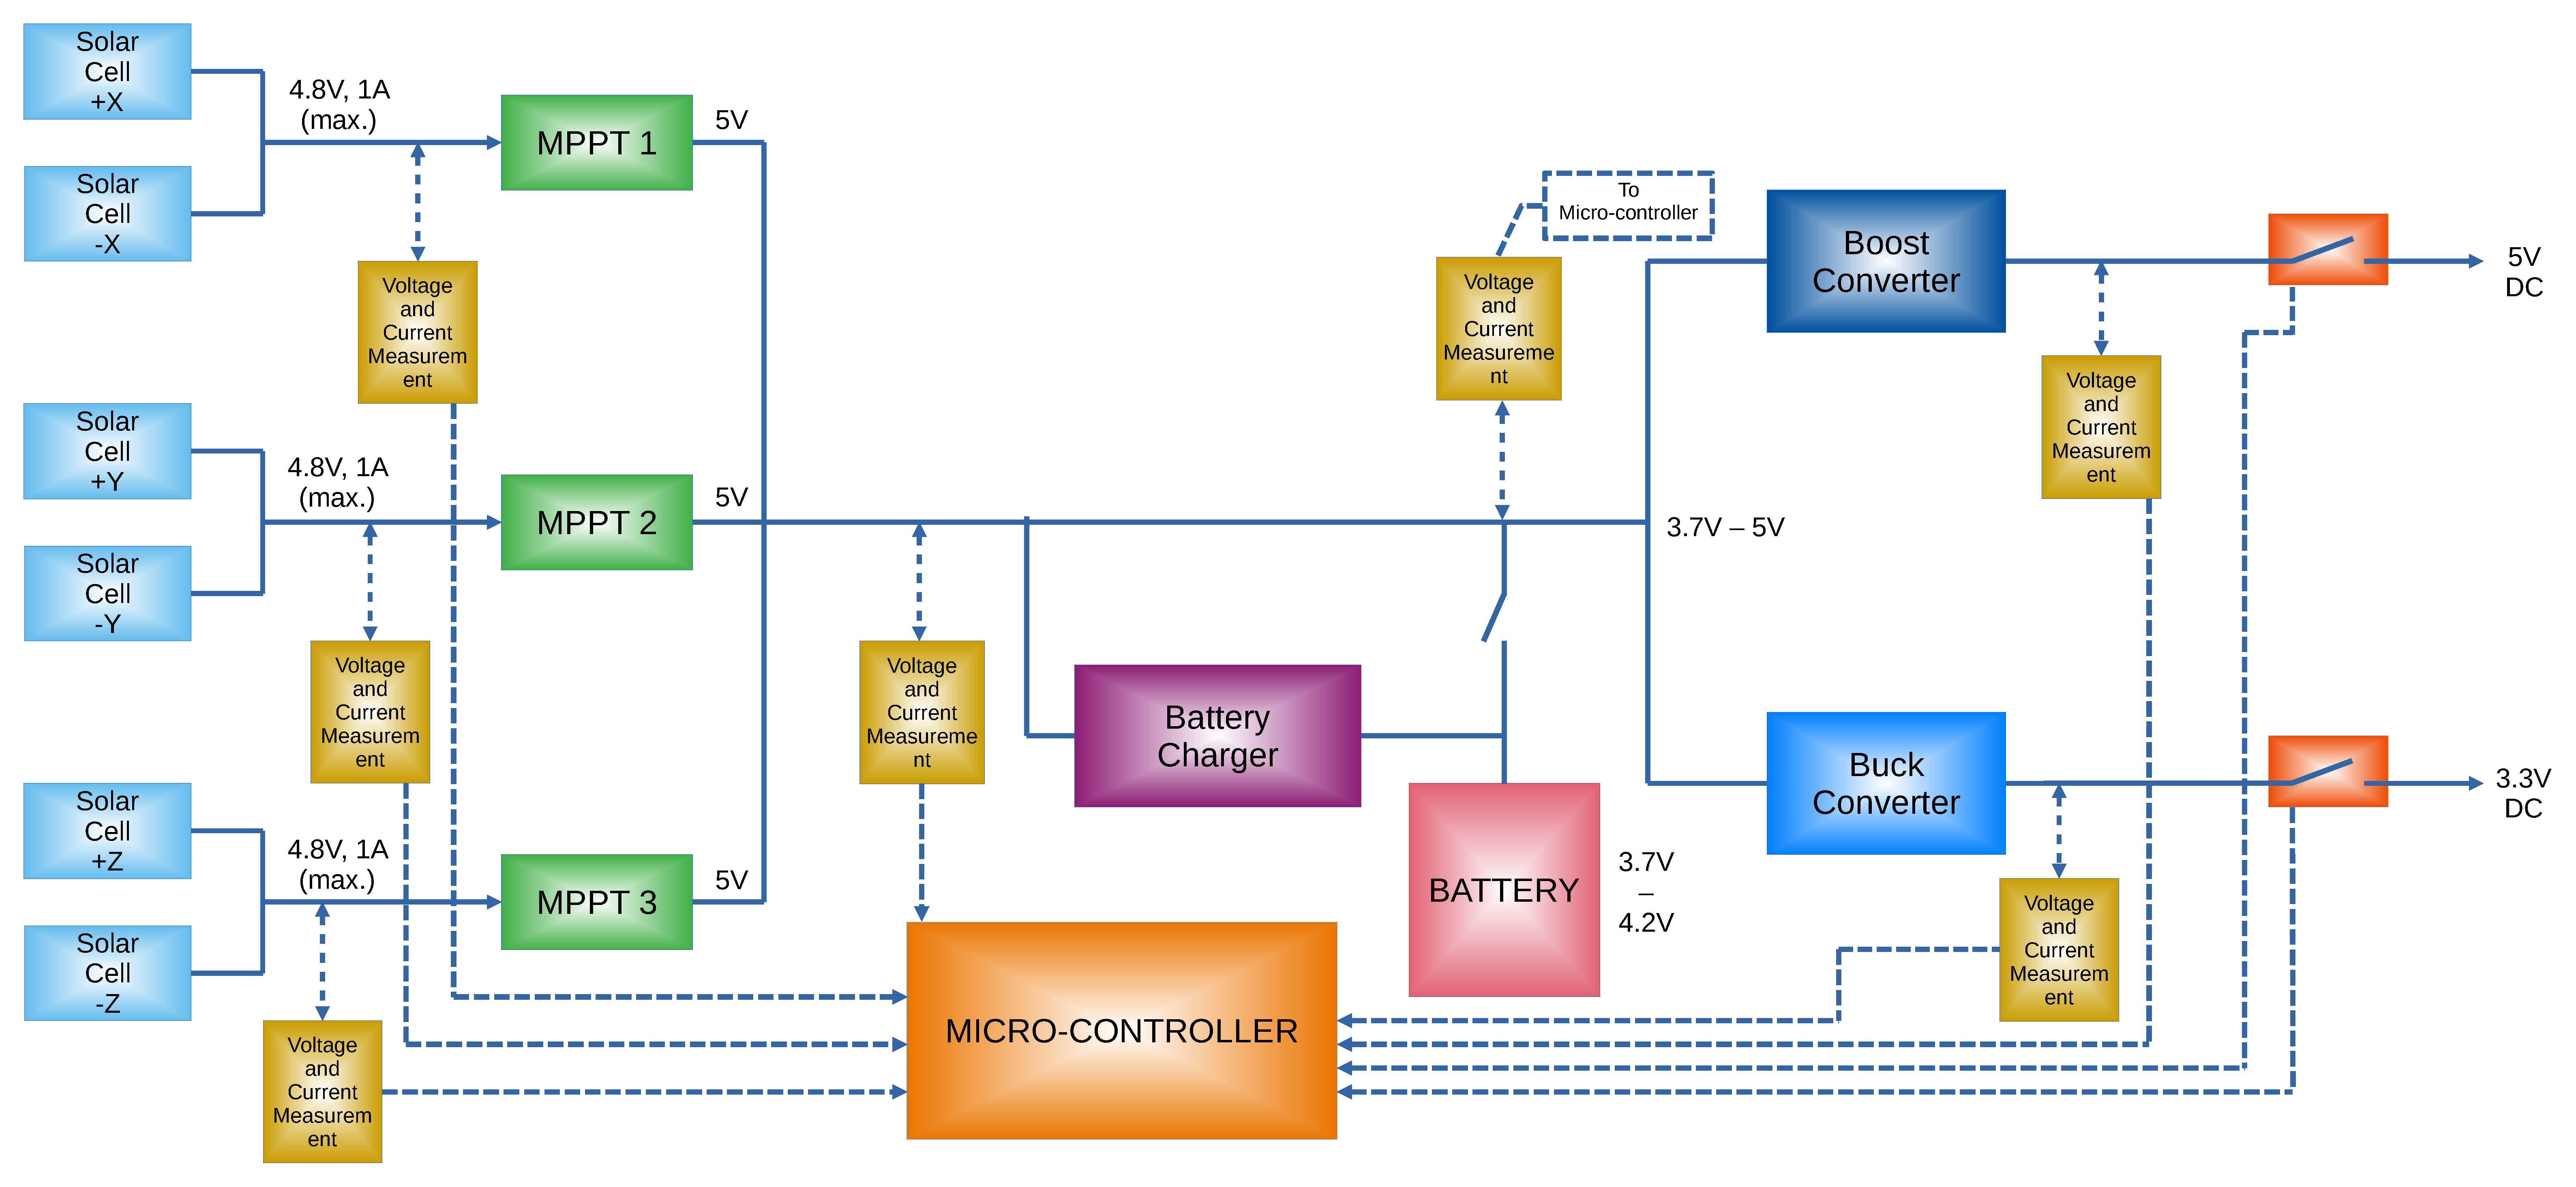
\includegraphics[width=\columnwidth]{IMGS/diag11.pdf}
		\caption{System Architecture of the CubeSat EPS}
		\label{fig:mainarch}
	\end{figure} 
\end{landscape}